\begin{answer}
    \begin{figure}[H]
        \centering
        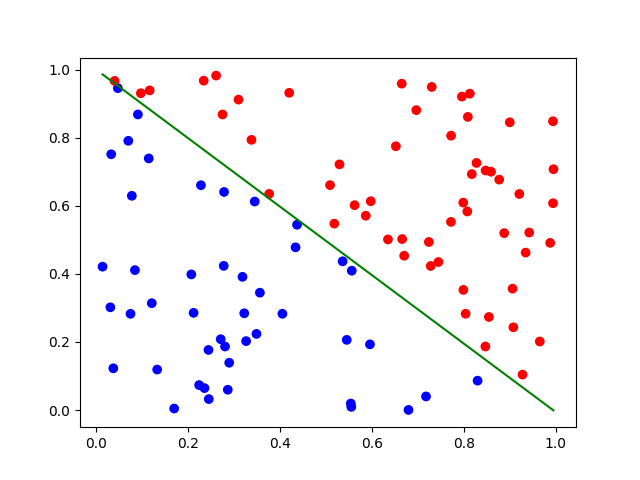
\includegraphics[width=0.6\textwidth]{src/logreg_stability/logreg_pred_b_no-reg.png}
        \caption{LR decision boundary for dataset B}
    \end{figure}

    \textbf{A:}
\begin{itemize}
    \item Seems to oscillate between two points while converging 
        \begin{itemize}
            \item Change in parameters $\theta$ from iter $>$ 5000 (constant (roughly)), while the loss stays constant
        \end{itemize}
    \item Loss stays relatively high (because points not linearly separable)
\end{itemize}

\textbf{B:}
\begin{itemize}
    \item Quickly converges to a very small loss $J(\theta) < 2$, whereas 
    \item Model parameters seem to grow continuously, steadily, while loss also sinks -- but both slowly in the range of $10^{-3}$ per iteration.
\end{itemize}

\vspace{1em}
\textbf{A vs. B:}

A seems to be inseparable in comparison to B, where you can draw a clear cut.

That is the reason why B's parameters explode -- the model gets too confident! The only way to lower the loss $J(\theta)$, is to maximize the term $\log(h_\theta(x))$, or minimize in case of $y=1$ $\log(1 - h_\theta(x))$. This is why the parameters take high values! As the exponential function in $h_\theta(x)$ never reaches 0 and is strictly increasing/decreasing, the loss will sink continuously

This is not the case with dataset A, as the loss has, due to its inseparability, a linearwise asymptote, and starts to oscillate around that median between the two configurations of $\theta$. \\

The logs at \href{run:./src/logreg_stability/logs_a.txt}{logs\_a.txt} and \href{run:./src/logreg_stability/logs_b.txt}{logs\_b.txt} are evidence of my findings.

\end{answer}
